\section{Evaluation}
\label{sec:eval} 
\paragraph{LLMs and PEFT models.} We evaluated \sys across three publicly available LLMs: \llama-3.1-8B~\cite{llama2}, Qwen-2.5-14B~\cite{qwen2025qwen25technicalreport}, and Qwen-2.5-32B~\cite{qwen2025qwen25technicalreport} from HuggingFace~\cite{huggingfacemodels}.
Since existing LLM serving systems only support base models and LoRA-based \peft, we focus on these configurations for fair comparison.
We applied LoRA with rank 16 to MLP down projection layers, yielding 9.4M, 14.5M, and 25.16M trainable parameters respectively.

\paragraph{Platform.} Experiments were performed on Perlmutter~\cite{perlmutter} nodes with AMD EPYC 7763 processors, \SI{256}{GB} DRAM, and four NVIDIA A100-SXM4-80GB GPUs connected via HPE Slingshot (\SI{200}{Gb/s}). We used tensor-model parallelism for LLM serving and finetuning.

\paragraph{Workload.} 
We synthesized inference workloads using ShareGPT~\cite{sharegpt} prompt/generation lengths and Azure ChatGPT production traces~\cite{burstgpt} for realistic arrival patterns, following recent work~\cite{10.1145/3600006.3613165, zhong2024distserve, agrawal2023sarathi, nanoflow, pipellm, medusa}. The original trace spans multiple days and captures real production arrival patterns from ChatGPT serving on Azure OpenAI, providing realistic inference workload characteristics including bursty request arrivals and varying concurrency patterns.  We sampled 20-minute intervals, adjusting the arrival times to simulate different average arrival rates.
We set TPOT SLOs to 50ms (8B model) and 75ms (14B/32B models) following the methodology from prior work~\cite{agrawal2023sarathi}, with 5s maximum TTFT to prevent excessive queueing.

We sampled each finetuning request from the \texttt{Sky-T1\_data\_17k} dataset~\cite{novasky2025dataset}, used to finetune the \texttt{Sky-T1-32B-Preview} reasoning model~\cite{novasky2025model}, a finetuned Qwen2.5 variant with performance comparable to OpenAI's o1-preview~\cite{o1-preview} on math and coding benchmarks. We truncated sequences to 8192 tokens and used the Adam optimizer~\cite{kingma2014adam}.

\subsection{End-to-end Comparison}

We compare \sys's co-serving approach with existing approaches that employ separate clusters for inference and finetuning tasks. In the separate cluster approach, we use vLLM~\cite{10.1145/3600006.3613165} and LlamaFactory~\cite{llamafactory} as the inference and finetuning systems, respectively, as they represent state-of-the-art solutions for these workloads. We selected vLLM over alternatives like DeepSpeed-MII~\cite{deepspeed-mii} and TensorRT-LLM~\cite{tensorrt-llm} because recent vLLM optimizations have closed previous performance gaps, while PipeSwitch~\cite{bai2020pipeswitch} lacks support for autoregressive LLM generation. We enable all available optimizations, including \texttt{torch.compile}, and chunked prefills for vLLM v1; DeepSpeed ZeRO Stage 3, Unsloth and FlashAttention for LlamaFactory.
We allocated 4, 8, and 16 A100 GPUs for the three models respectively.

\Cref{fig:end-to-end} shows the results. The separate approach uses tensor parallelism (degree 1, 2, 4) for the three models respectively, creating four pipelines in total. We explored various strategies to distribute resources between inference and finetuning tasks. Configurations like 25\% vLLM - 75\% LlamaFactory allocate 25\% of resources (i.e., 1 pipeline) to inference, 75\% (i.e., 3 pipelines) to finetuning.

Configurations with fewer inference pipelines (25\%-50\% vLLM) handle only lightweight workloads, achieving limited inference throughput and SLO attainment under more intensive workloads. Dedicating more pipelines to inference (75\% vLLM) maintains high SLO attainment but reduces finetuning throughput.

\Sys maintains near-optimal SLO attainment without compromising finetuning performance by prioritizing latency-sensitive inference and opportunistically maximizing finetuning tokens.

Across all three models, \sys matches the 75\% vLLM - 25\% LlamaFactory configuration in inference SLO attainment (at or above 90\% even at 20 req/s) and inference throughput, while dramatically improving finetuning throughput. Specifically, under heavy inference loads (20 req/s), \sys sustains finetuning throughputs of 7.2K, 2.2K and 2.2K tokens/s for LLaMA-3.1-8B, Qwen-2.5-14B, and Qwen-2.5-32B respectively, compared to only 3.8K, 1.0K, and 0.5K tokens/s in the 75\% vLLM - 25\% LlamaFactory setup—i.e. a \textbf{1.9$\times$-4.8$\times$} improvement. Under light inference loads (4.0 req/s), \sys sustains finetuning throughputs of 9.4K, 3.7K, and 3.2K tokens/s for the same models, translating to a \textbf{2.5$\times$-6.8$\times$} improvement over the 75\% vLLM - 25\% LlamaFactory setup.


\subsection{GPU Scheduling}

This section compares \sys's co-serving mechanism with two commonly used GPU scheduling strategies: {\em temporal sharing} and {\em spatial sharing}. 
Temporal sharing interleaves the execution of inference and finetuning tasks over time, as illustrated in \Cref{fig:baseline}. Spatial sharing simultaneously launches inference and finetuning computations using separate CUDA resources. Both strategies are implemented on top of \sys by replacing the co-serving mechanism with their respective scheduling strategies. To ensure a fair comparison, all memory optimizations are enabled in each baseline. 

\Cref{fig:temporal-spatial-sharing} shows the results. For temporal sharing, interleaving one inference iteration with one finetuning iteration would violate the SLOs for nearly all inference requests.
This is because each inference iteration is expected to complete within tens of milliseconds, whereas a finetuning iteration requires several seconds. To mitigate this issue, in the temporal sharing experiments, we interleave each finetuning iteration with $n$ inference iterations, where $n$ is the inference frequency shown in the figure.

While adopting a low inference frequency in temporal sharing (i.e., frequency = 64) maximizes finetuning throughput, it adversely impacts the SLO attainment and throughput for inference requests.
Employing a frequency of 128 enables temporal sharing to match the inference throughput and SLO attainment rate of co-serving. However, it also reduces finetuning throughput by 0.57x-0.86$\times$ compared to co-serving.

Finally, we also implemented a dynamic temporal sharing baseline (see \Cref{sec:dts-appendix}), where the interleaving frequency is determined dynamically based on queue lengths, batch sizes, arrival rates, and completion rates.
Dynamic temporal sharing outperforms fixed-frequency temporal sharing by adapting to workload conditions, maintaining SLO attainment above 90\% in most scenarios, and achieving impressive inference throughputs of 5.4K, 4.9K, and 6.6K tokens/s for the three models under heavy loads (20 req/s). However, it still lags behind co-serving, whose finetuning throughput is \textbf{1.0–1.7$\times$} higher, and shows instability under the heaviest loads as SLO attainment drops significantly for the 32B model.

Spatial sharing allocates separate GPU resources for inference and finetuning, achieving comparable finetuning throughput to co-serving. However, it remains suboptimal in SLO attainment under heavy inference workloads due to the interference between inference and finetuning tasks.

\begin{figure}[t]
    \centering
    \begin{subfigure}[b]{\linewidth}
      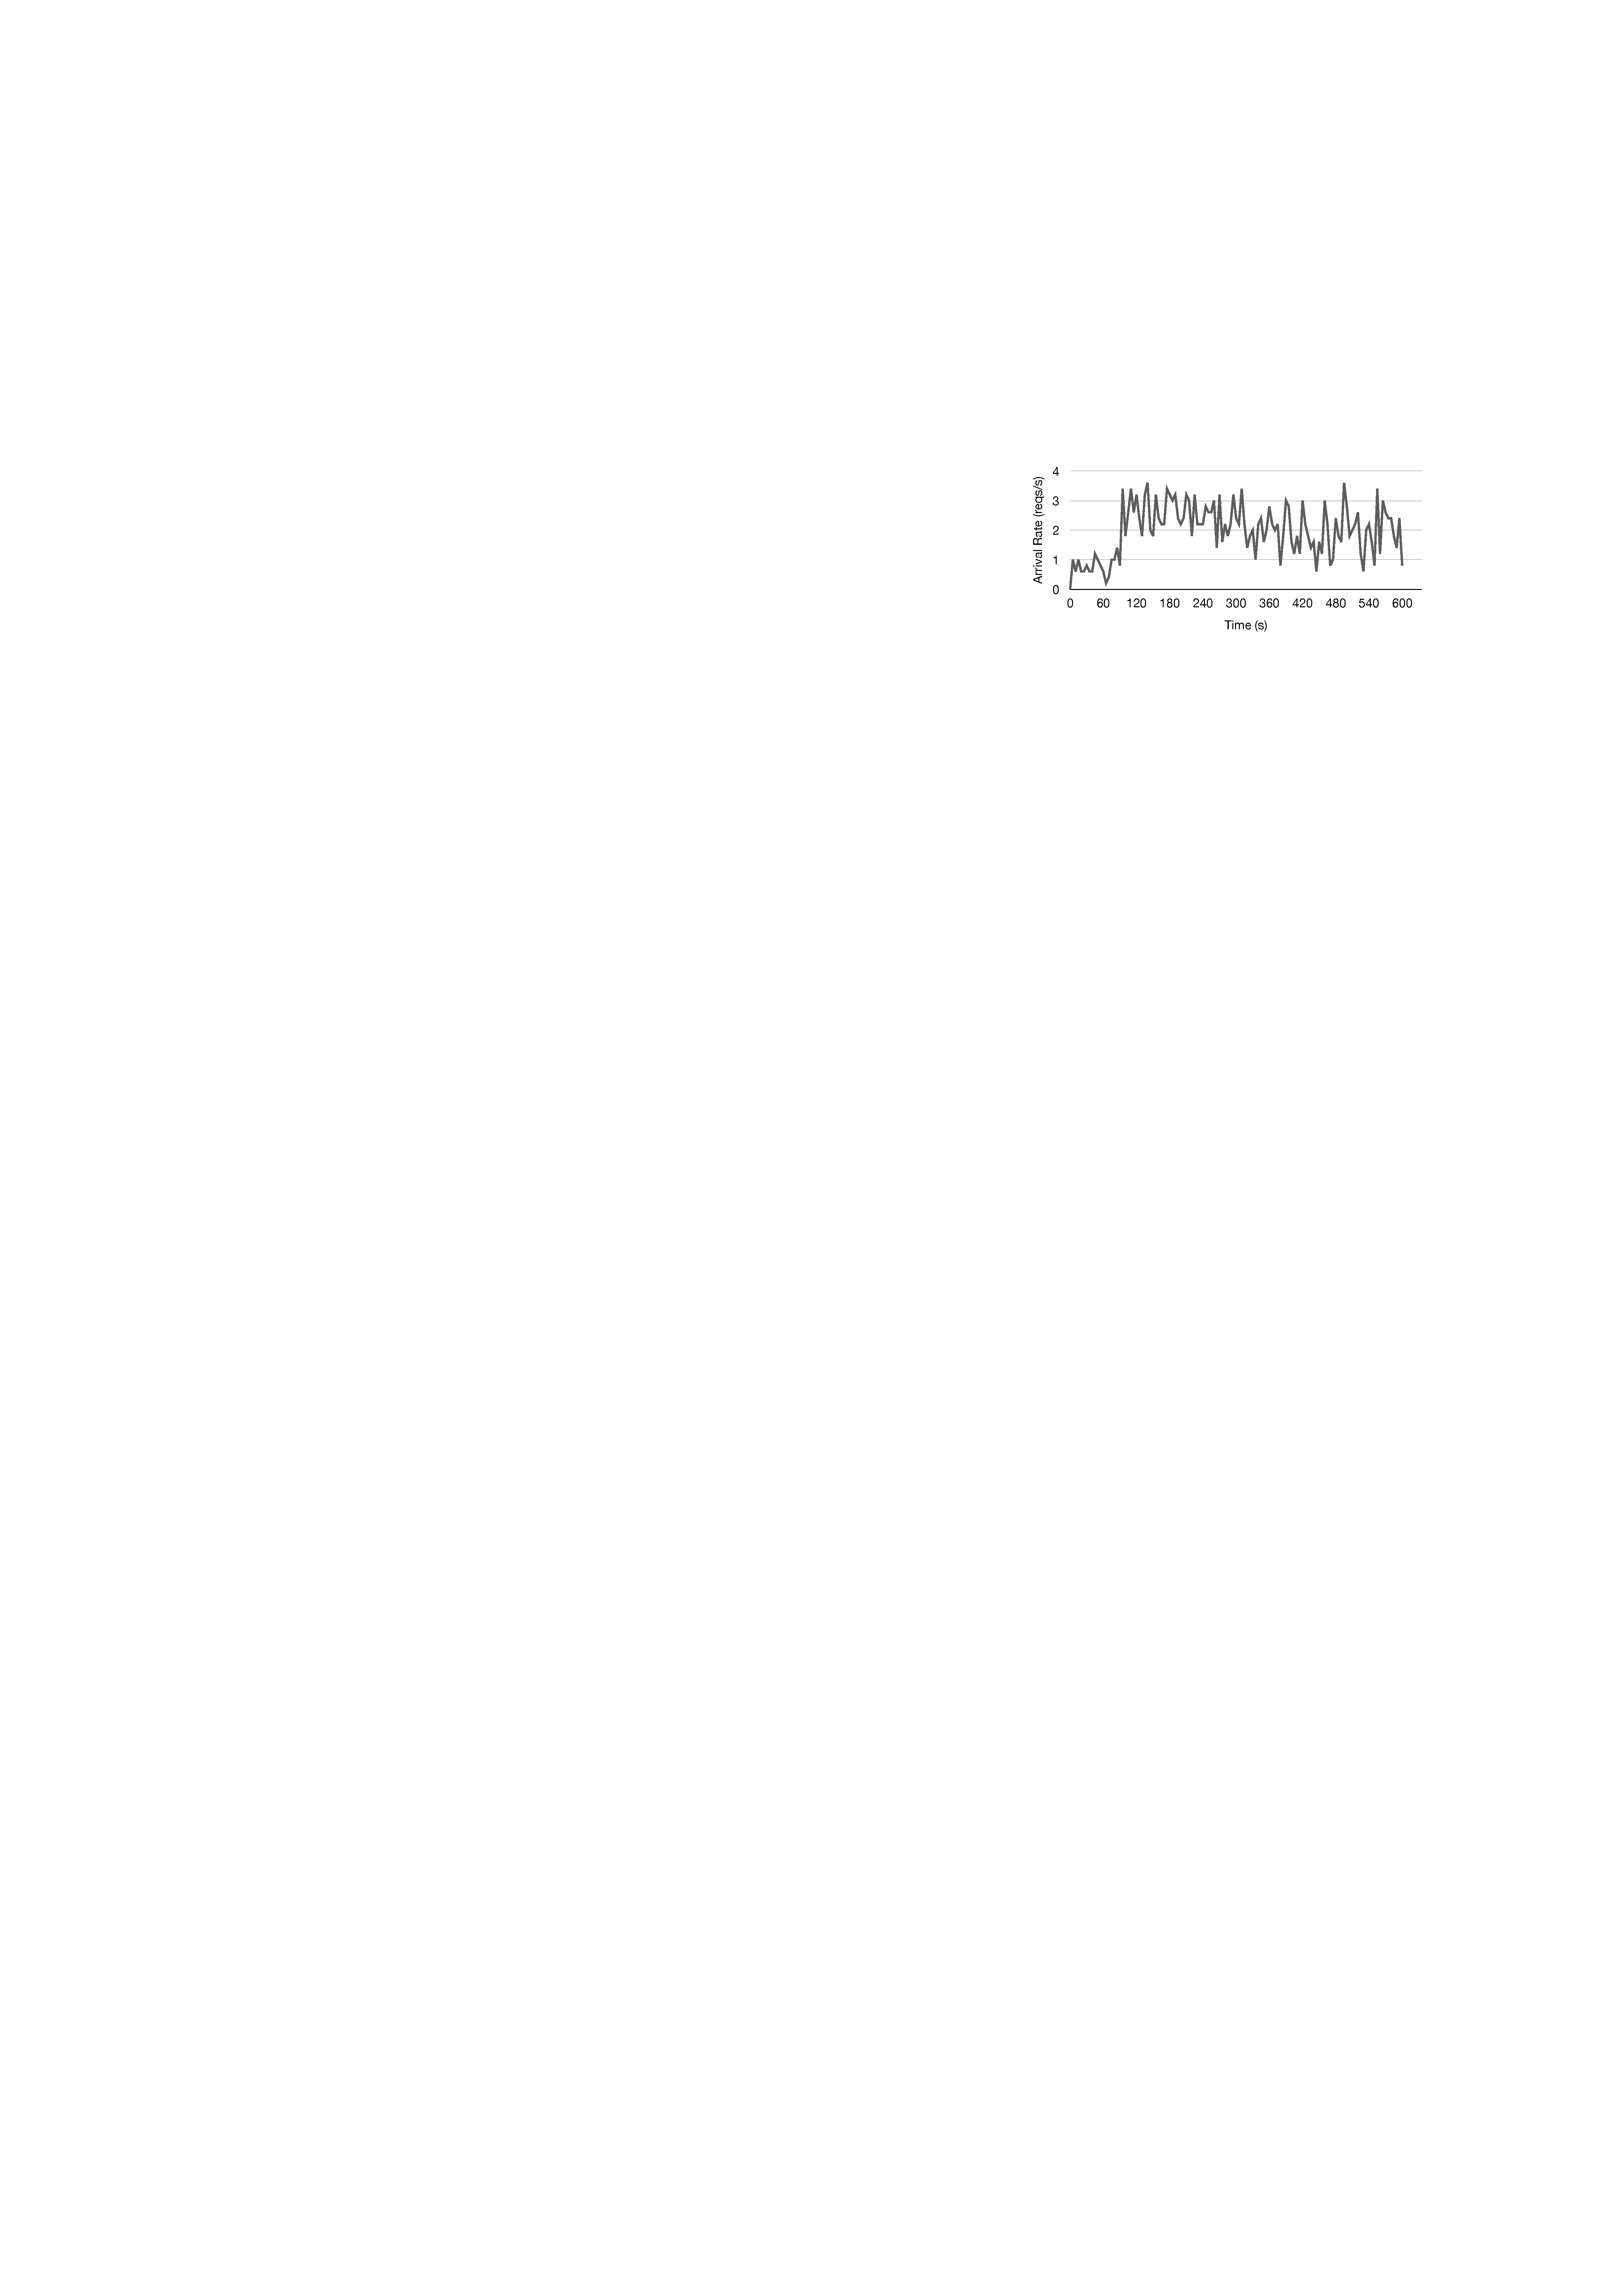
\includegraphics[width=\linewidth]{figs/case_arrival.pdf}
      \caption{Arrival Inference Requests}
    \end{subfigure}\\ 
    \centering
    \begin{subfigure}[b]{\linewidth}
      \centering
      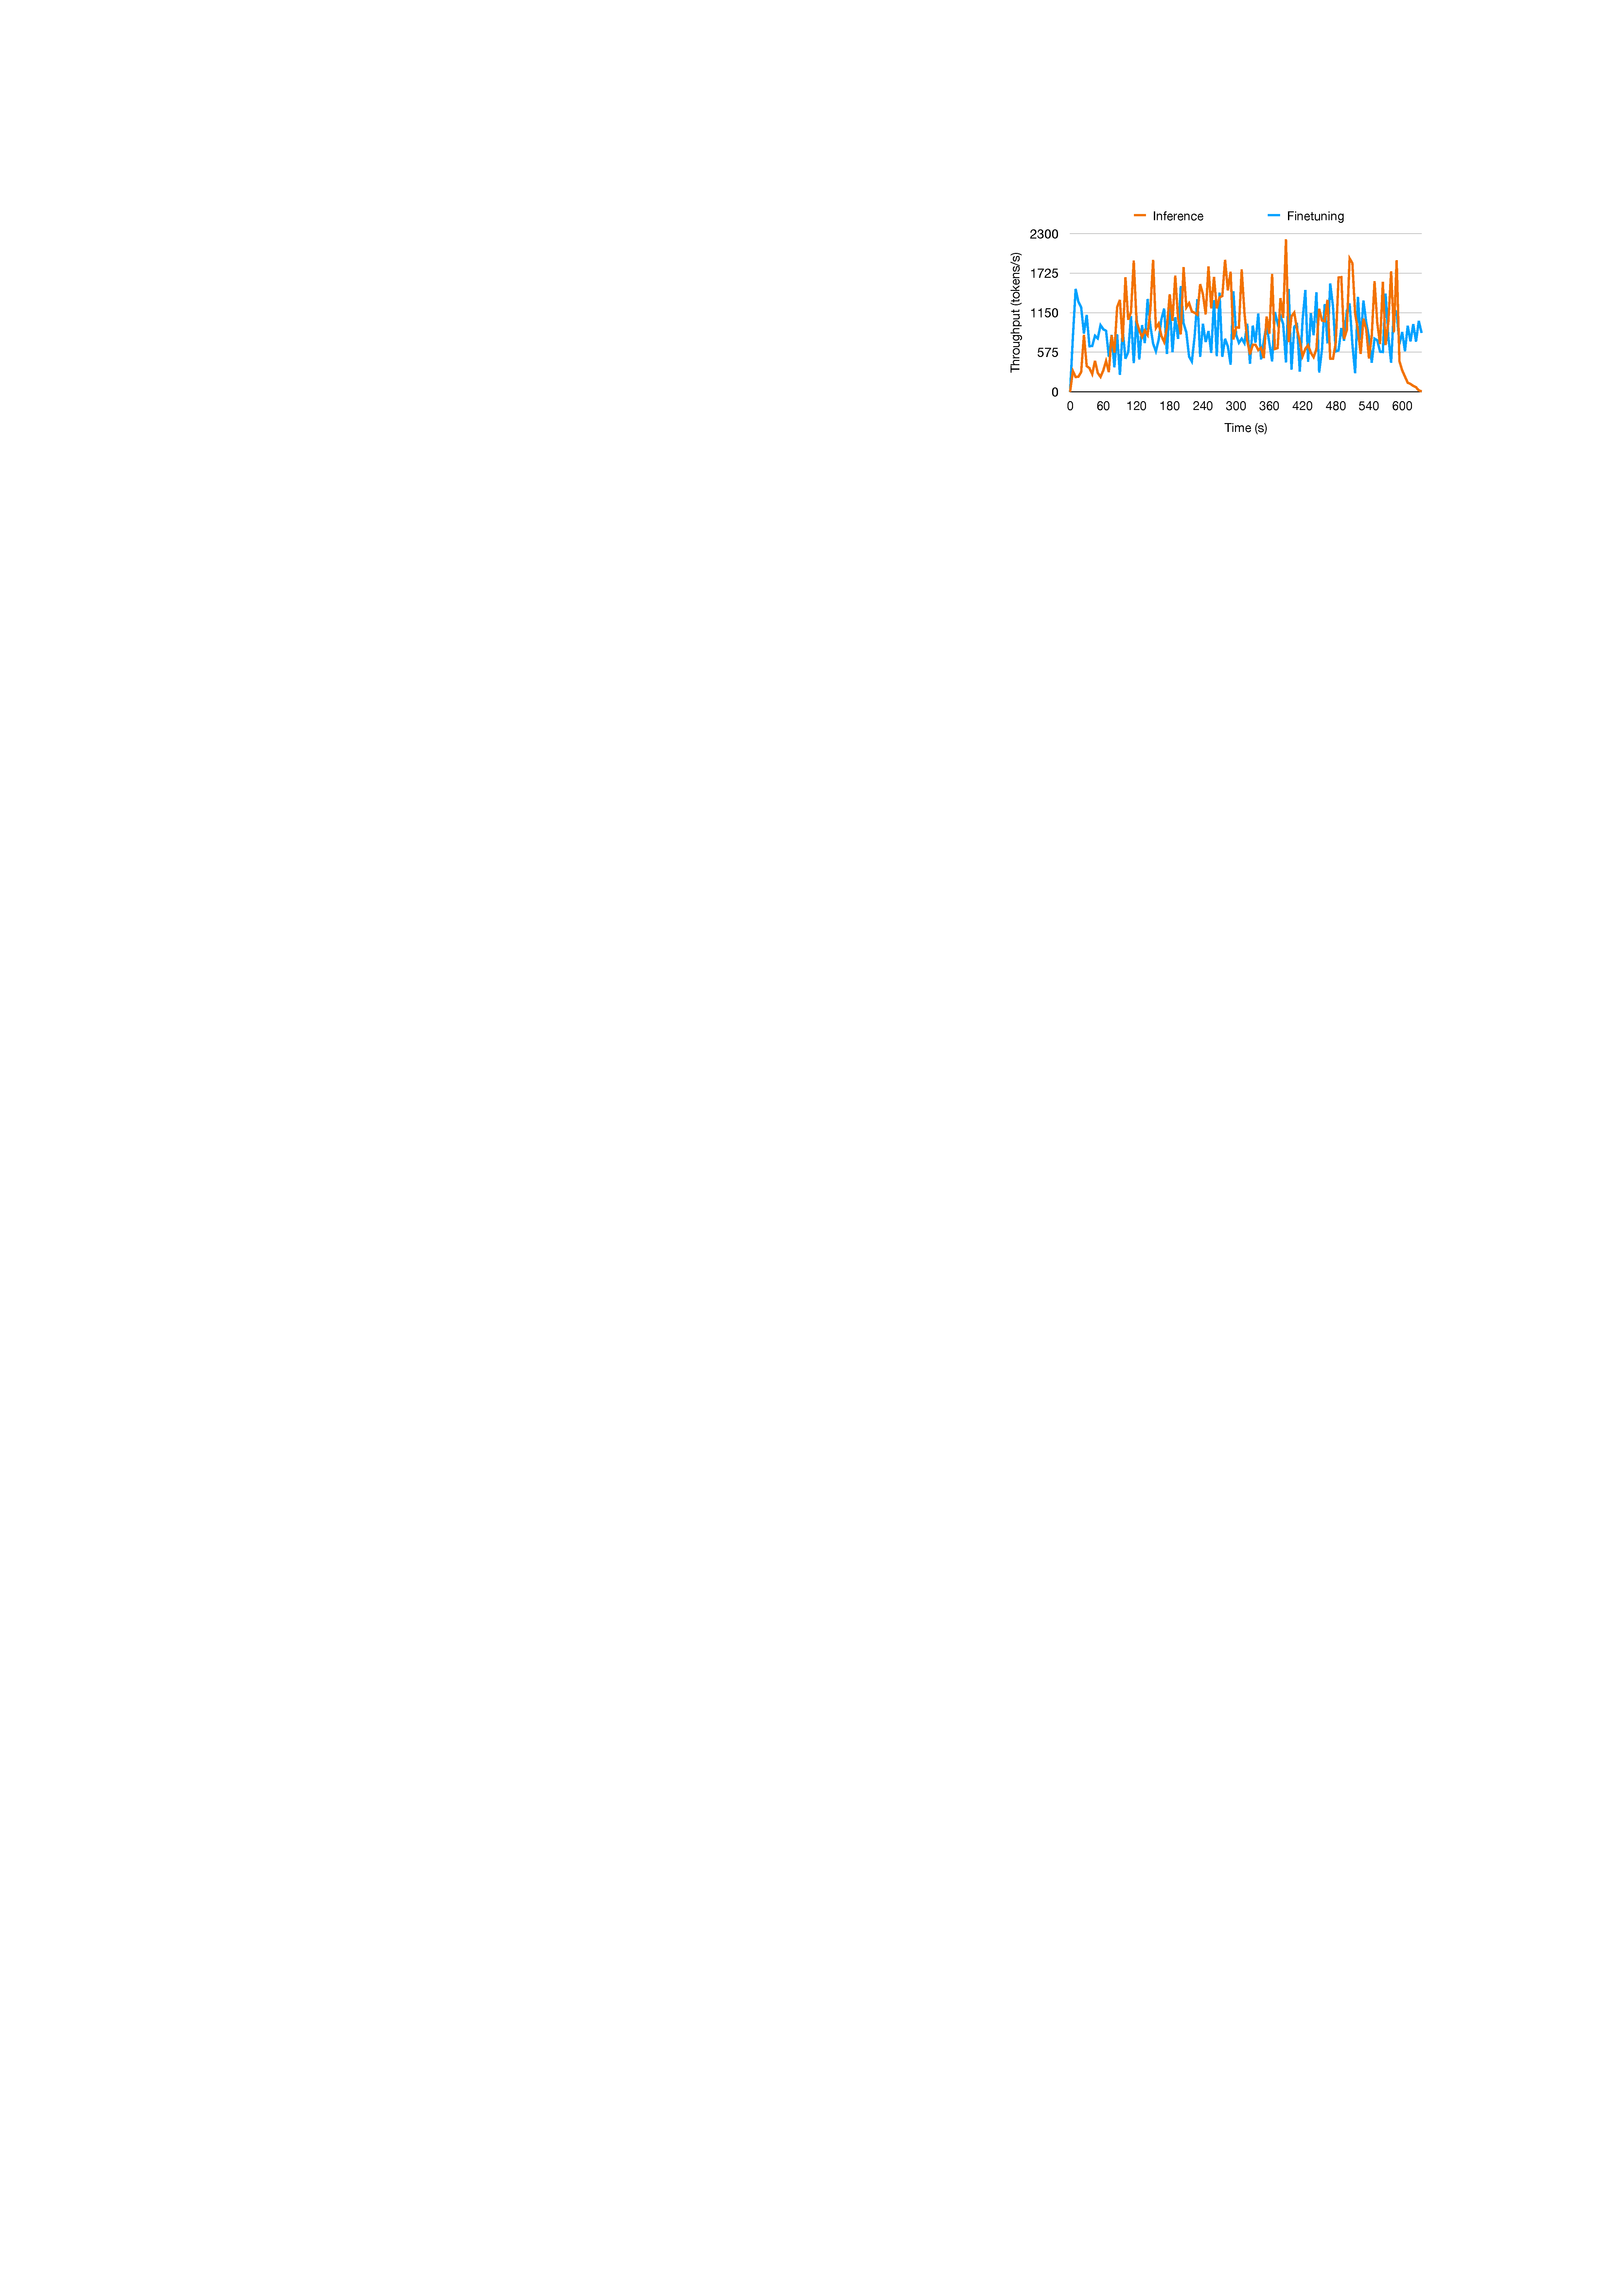
\includegraphics[width=\linewidth]{figs/case_tpt.pdf}
      \caption{System throughput}
    \end{subfigure}
  \caption{Case study of \sys's system throughput for fluctuating inference workload.}
  \label{fig:case_study}
\end{figure}

\subsection{Case Study}
\label{sec:exp:dynamic}
This case study demonstrates \sys's ability to dynamically adapt to fluctuating inference workloads in real-time. We evaluate \sys using a 10-min interval of the BurstGPT trace with Qwen-2.5-14B model. To ensure compatibility with our experiment environments, we replayed this trace segment and re-scaled its arrival intensity, as previous works have done~\cite{285173,258862,ali2022optimizing,miao2023spotserve}. In the experiment, each inference request and inference request are sampled from the ShareGPT dataset and the Sky-T1 dataset respectively.

In our case study, as shown in Figure~\ref{fig:case_study}, we observed that the arrival rate of the inference requests initially increased to a peak level after around 90 seconds, and then gradually decreased with some peaks. \sys could automatically detect the fluctuations in the workload and improve the ratio of inference tokens (vs finetuning tokens) in each iteration's batch. This significantly increased inference throughput from a few hundreds to 2.25K.

\subsection{Memory Optimization}
\label{eval:memory_optimization}
\begin{figure}[t]
    \centering
    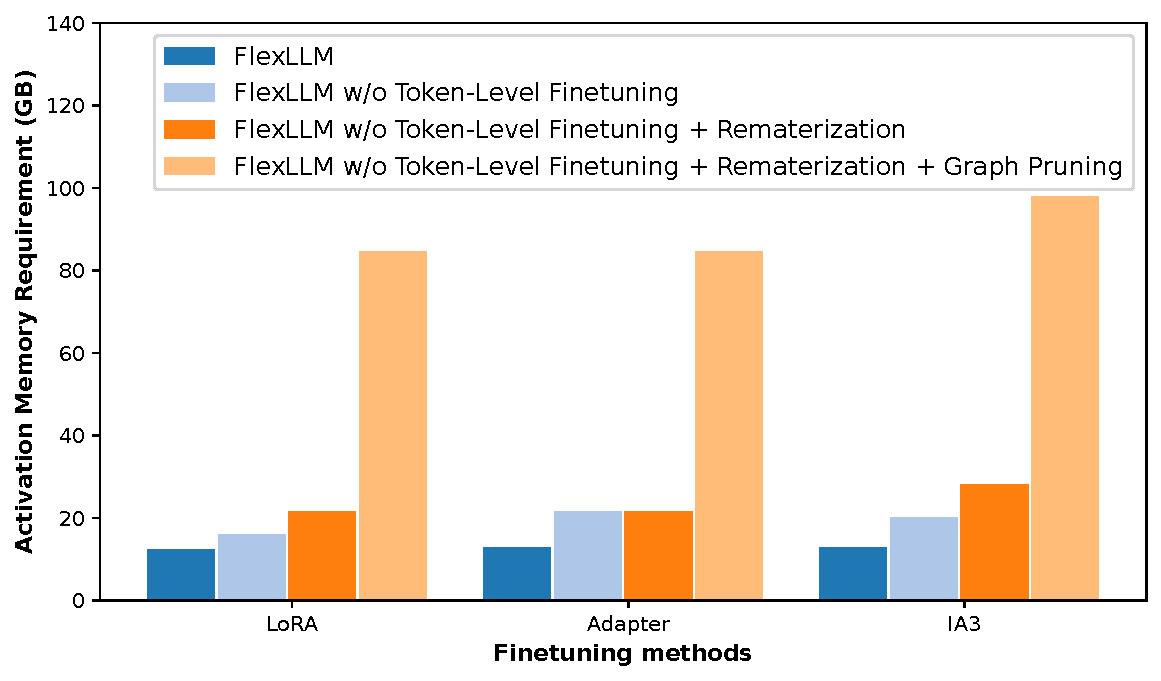
\includegraphics[width=0.85\linewidth]{figs/fig_memory_act3.pdf}
    \caption{Ablation study of memory optimizations.}
    \label{fig:memory_ablation}
\end{figure}

\sys introduces a series of memory optimizations to reduce the memory overhead of \peft finetuning and allow co-serving finetuning with inference workloads.
%
To understand the effectiveness of \sys memory optimizations, we perform an ablation study that incrementally turns off these optimizations (graph pruning, rematerialization, and token-level finetuning) and measures the memory requirements. 
%
\Cref{fig:memory_ablation} shows the activation memory requirements of \sys for different finetuning methods on a 70B LLM and a sequence length of 1024. \sys saves $85\%$-$87\%$ memory requirements for activations compared to existing approaches. The major improvement comes from graph pruning. With graph pruning only, \sys achieves $71\%$-$74\%$ activation memory overhead reduction. Rematerialization and token-level finetuning further reduce memory overhead by $0$-$8\%$ and $4\%$-$10\%$, respectively. These memory optimizations are highly effective in practice, enabling \sys to retain sufficient memory for the inference requests' KV cache, ensuring eviction rates of 0\% in most cases and peaking at only 1.2\% for the largest model (Qwen2.5-32B) under the heaviest loads (see \Cref{sec:coserving_evictions}).

